\chapter{Soluci\'on propuesta}
\label{chap:sol}
%\porHacer{Figuras pendientes (diagramas de clases sobretodo). Algunas secciones necesitan reestructuraci\'on. (10 d\'ias desde hoy aprox.)}

El objetivo principal de este trabajo es proporcionar una t\'ecnica que permita buscar pistas que se relacionen por su ritmo real. Mediante un software programado en {\sc Python}, se realizan las tareas de analizar archivos de sonido y guardar la informaci\'on de ritmo en archivos de datos. La implementaci\'on de este software consiste principalmente en tres partes; la reproducci\'on, que se lleva acabo en un {\em hilo}\footnote{Un {\em hilo} es una unidad de procesamiento que permite al software ejecutar tareas en paralelo.} separado que solo se encarga de leer fragmentos de sonido y reproducirlos; el an\'alisis, se realiza en otro hilo que toma informaci\'on del fragmento actual reproducido y la selecci\'on de pista, que corre en el mismo hilo que el an\'alisis y se encarga de seleccionar la mejor pista candidata a ser reproducida.

\section{Metodolog\'ia}

En el cap\'itulo anterior se mencionan las caracter\'isticas principales del proyecto y se hace una comparaci\'on con trabajos relacionados. Ahora se discuten los procedimientos necesarios para lograr el funcionamiento propuesto y las herramientas utilizadas para el proyecto.

\subsection{Planeaci\'on de proyecto}
Para comenzar con el desarrollo del proyecto es necesario hacer una selecci\'on de herramientas. Se seleccion\'o el lenguaje de programaci\'on {\sc Python}\footnote{{\sc Python} es un lenguaje de programaci\'on prop\'osito general de alto nivel.} debido a su facilidad de uso, con el cual se puede lograr hacer prototipos funcionales en poco tiempo. 

\noindent Dentro de las librer\'ias utilizadas, se mencionan aquellas que permiten lograr el an\'alisis necesario. Por defecto {\sc Python} incluye varios m\'odulos que permiten la manipulaci\'on de se\~nales provenientes de archivos de sonido.

\noindent {\sc Python} incluye en su librer\'ia estandar el m\'odulo {\sc wave}\footnote{El m\'odulo {\sc wave} proporciona una interfaz conveniente para la manipulaci\'on de archivos WAV.} que hace posible la manipulacion de archivos en formato WAV\footnote{WAV es un formato de audio digital generalmente sin compresi\'on.} sin compresi\'on. Tambi\'en incluye el m\'odulo {\sc audioop}\footnote{El m\'odulo {\sc audioop} proporciona operaciones para la manipulaci\'on de fragmentos de audio.} con la cual se puede hacer varias modificaciones a los fragmentos generados por el m\'odulo {\sc wave} tales como sumar dos fragmentos, aumentar la intensidad de los mismos, entre otras operaciones.                        

\noindent Tambi\'en se utilizaron librerias de terceros que facilitan la tarea de an\'alisis. Para poder reproducir los fragmentos de sonido en un archivo se utiliz\'o la librer\'ia {\sc PyAudio}\footnote{{\sc PyAudio} es una librer\'ia de {\sc Python} para la reproducci\'on y grabaci\'on de flujos de audio}. Adem\'as se utiliz\'o la librer\'ia {\sc NumPy}\footnote{{\sc NumPy} es una librer\'ia de {\sc Python} que agrega mayor soporte para matrices y vectores.} con la que es posible realizar el c\'alculo de la transformada r\'apida de Fourier con la que se obtiene la intensidad de cada frecuencia en una pista.

\subsection{M\'etodo de procesamiento}

La intenci\'on del procesameinto de se\~nales en este proyecto es obtener el tempo de la pista en reproducci\'on. Para ello primero se procede a leer un archivo de sonido, en este caso se opt\'o por el formato WAV sin compresi\'on debido a su f\'acil manipulaci\'on sin la necesidad de utilizar librer\'ias de decodificaci\'on, sin embargo el proceso es facilmente adaptable a cualquier formato.

\noindent El modulo {\sc wave} permite la lectura de archivos en formato WAV de los cuales se obtiene una serie de fragmentos que corresponden a un instante de sonido. Mediante la librer\'ia {\sc PyAudio} se crea un flujo de lectura de estos fragmentos, esto reproduce el instante de sonido. El fragmento reproducido esta en formato PCM\footnote{La modulaci\'on por impulsos codificados (PCM del ingl\'es Pulse Code Modulation) es un procedimiento para transformar una se\~nal anal\'ogica a secuencias de bits.}  que describe la forma de la onda producida, con el fragmento es posible analizar una aproximaci\'on a la frecuencia independiente de cada sonido mediante el c\'alculo de una transformada r\'apida de Fourier.

\noindent Con las frecuencias obtenidas se procede a calcular una aproximaci\'on de tempo para lograr una detecci\'on de ritmo. En este contexto el tempo calculado no es fiel al t\'ermino real; para este contexto el tempo hace referencia a los sonidos reproducidos en el instante y no al instrumento espec\'ifico como se hace normalmente. La aproximaci\'on se logra calculando una diferencia entre las frecuencias actuales y las frecuencias del instante pasado; si la diferencia en una banda es muy amplia, \'esta influenciar\'a la decisi\'on de tomar el instante como un pulso o no. Finalmente la diferencia de tiempo entre pulsos define el tempo aproximado para el instante.

\subsection{M\'etodo de clasificaci\'on}

Los datos preprocesados de los archivos de sonido describen un ritmo algo espec\'ifico para el tipo de m\'usica que se reproduce. \'Estos contienen un inicio y un final casi siempre distintos, sin embargo es necesario detectar en que parte de la pista deja de ser el inicio y en que parte comienza el final de la misma. Por ello es necesario hacer una clasificaci\'on de datos.

\noindent Con una clasificaci\'on de datos es posible comparar inicio y final de dos pistas distintas pero que comparten similitudes en sus ritmos, estas similitudes son encontradas mediante un algor\'itmo de reconocimiento de patrones, en el que se analizan los datos preprocesados para buscar zonas en la pista que tengan un tempo que siga un patr\'on parecido en ambas pistas. De esta manera es posible difuminar el final de una pista donde el tempo es tentativamente distinto con el inicio de otra pista donde el tempo se iguala.

\noindent Los datos preprocesados consisten en arreglos de valores que representan tiempo en la pista e intensidad de pulso para el tiempo dado. El programa analiza los datos y compara cada valor de intensidad buscando repeticiones en su comportamiento; es decir, cuando los valores de intensidad suben y bajan en cierta medida respetando un rango especificado.

\section{Dise\~no e implementaci\'on}

En un principio se ten\'ia una combinaci\'on de elementos de interfaz con elementos algor\'itmicos; ciertos eventos de la interfaz controlaban algunas variables que el algoritmo utilizaba. Ahora el software trabaja con m\'odulos independientes, lo que inclusive permite implementar algunos de ellos en un lenguaje de programaci\'on distinto. Principalmente el software se compone por m\'odulos de interfaz que controlan los eventos de la misma y m\'odulos del algoritmo que simplemente ejecutan una tarea hasta terminarla, ademas se implementan conectores entre los m\'odulos de interfaz y los del algoritmo con el fin de comunicar a ambos de forma que no existan interferencias ni p\'erdidas de datos.

\subsection{Interfaz}

En la figura \ref{fig:inter} se muestra el dise\~no propuesto de la interfaz de acuerdo con el objetivo principal de la tesis. 

\begin{figure}[h!]
\centering
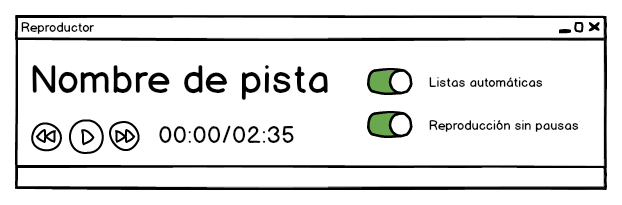
\includegraphics[width=15cm]{./Figuras/window}
\caption[Interfaz de usuario]{La interfaz de usuario utiliza controles simples para evitar complicaciones de uso.}
\label{fig:inter}
\end{figure}

\noindent El software tiene una interfaz simple, consta de un bot\'on de reproducci\'on/pausa y un par de botones para la pista siguiente y la anterior. Muestra una etiqueta para el nombre del archivo en reproducci\'on y una para el tiempo restante. Tambi\'en se tiene un par de botones para activar la generaci\'on de listas de reproducci\'on autom\'atica y la reproducci\'on sin pausa.

%\porHacer{M\'as elementos de interfaz se podr\'ian agregar en el futuro.} 

\subsection{Funcionamiento interno}

Las funciones principales del software son tres:

\begin{description}
\item[Reproducci\'on de archivos.]{La funci\'on b\'asica es la de reproducir archivos en formato {\sc WAV} sin compresi\'on.}
\item[Generaci\'on de listas de reproducci\'on.]{Un generador de listas basado en la inforaci\'on obtenida del procesamiento de cada archivo. Mediante un algoritmo de b\'usqueda de similitudes entre los datos se puede encontrar la siguiente pista a reproducir.}
\item[Transici\'on inteligente.]{Al estar activa la opci\'on de reproducci\'on sin pausa, las pistas tendr\'an una trnasici\'on suave entre inicio y fin. La selecci\'on de los puntos de transici\'on se hace mediante un algoritmo que reconoce un punto entre dos pistas que tiene un ritmo que sea semejante.}
\end{description}

\noindent En la figura \ref{fig:func} se muestra un diagrama del funcionamiento del software.

\begin{figure}[h!]
\centering
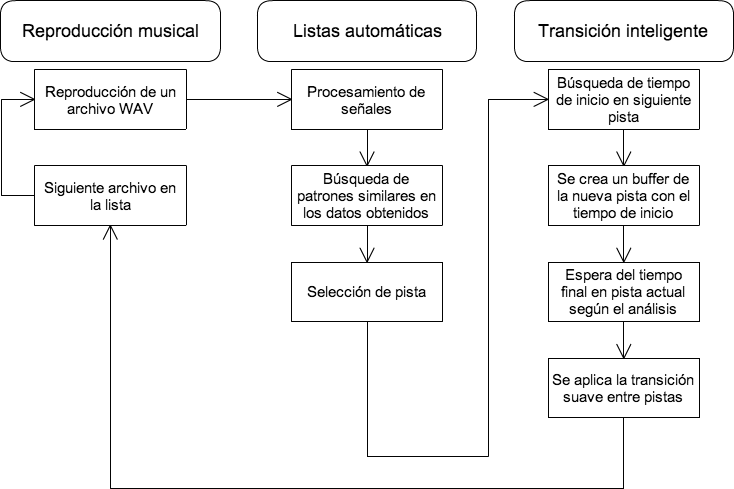
\includegraphics[width=15cm]{./Figuras/diagram1}
\caption[Funcionamiento del software]{Funciones principales del software.}
\label{fig:func}
\end{figure}

\section{Obtenci\'on de informaci\'on relevante}

Para poder generar una lista de reproducci\'on basada en el ritmo de las pistas es necesario procesar \'estas antes. Para ello es necesario utilizar la transformada r\'apida de Fourier con la cual se obtiene informaci\'on de las frecuencias individuales en un tiempo $t$. El proceso de obtenci\'on de informaci\'on relevante consiste en capturar en ventanas de tiempo constantes la informaci\'on de las frecuencias, al t\'ermino de cada ventana de tiempo se hace una selecci\'on l\'ogica por medio de votaciones. Los valores en tiempo $t_1$ mayores a los del tiempo $t_0$ dan un voto positivo, los menores dan un voto negativo, al final se cuentan los votos de la ventana de tiempo y si la mayor\'ia son positivos entonces se almacena el valor actual, de no serlo simplemente se continua a la pr\'oxida ventana de tiempo.

\noindent La l\'ogica anterior se basa en que la pista presenta intensidades propias de su ritmo, la intenci\'on es capturar los momentos en que ocurre un cambio de intensidades para comparar con otras pistas y encontrar aquellas que sean compatibles en ritmo.

\noindent Ya que al reproducir una pista es necesario obtener de ella sus datos en formato PCM, \'estos se utilizan para realizar el proceso de obtenci\'on de informaci\'on en forma paralela a la reproducci\'on, cada instante de tiempo se actualizan estos datos, de esa manera se asegura que el tiempo de obtenci\'on sea equivalente al de la pista. Los datos obtenidos se almacenan en un archivo de texto plano.

\begin{landscape}
\begin{figure}
\centering
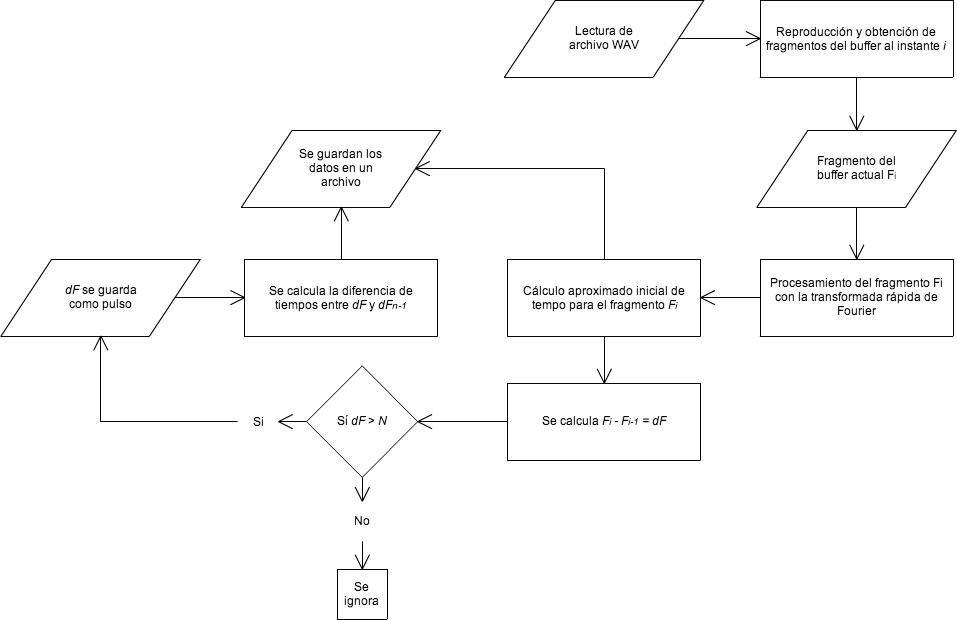
\includegraphics[width=22cm]{./Figuras/diagram2}
\caption[Obtenci\'on de informaci\'on]{Obtenci\'on de informaci\'on relevante de la pista.}
\label{fig:diaginfo}
\end{figure}
\end{landscape}

\section{Generaci\'on de listas de reproducci\'on}

La selecci\'on de pistas se realiza mediante un an\'alisis de datos que corre en paralelo con la reproducci\'on actual. Cada pista que se reproduce tiene un archivo de informaci\'on obtenida y se utiliza para comparar la pista correspondiente con las pistas en el directorio. La rutina que compara los datos entre pistas consiste en buscar un patr\'on de comportamiento en los datos, primero se buscan patrones en el archivo de datos de la pista en reproducci\'on, es decir, buscar secciones en los datos que sean coincidentes, se almacena el patr\'on y se guardan los tiempos en que ocurre el patr\'on encontrado. Con esa informaci\'on se procede a analizar los archivos de datos de las pistas en el directorio, por cada an\'alisis se realiza una rutina de comparaci\'on entre los datos de la pista actual $p_r$ y los de la candidata $p_c$. El an\'alisis consiste en comparar los datos de ambas pistas de tal manera que sigan un patr\'on de subidas y bajadas en los valores de los datos; si el valor de $p_{ri}$ y el valor de $p_{ci}$ son al mismo tiempo mayores o menores que $p_{ri-1}$ y $p_{ci-1}$ respectivamente entonces los patrones son compatibles y se procede a comparar los siguientes valores, en caso de que $p_{ri-1}$ sea mayor que su valor anterior y $p_{ci-1}$ menor al suyo entonces el patr\'on ya no es aceptable si se procede a analizar a otro patr\'on.

\noindent Con esa informaci\'on se obtienen los tiempos donde hay patrones compatibles entre la pista actual y la candidata, ahora solo queda seleccionar el que mejor se adapte. Normalmente cada pista tiene varios patrones candidatos, el mejor de ellos debe tener un equilibrio entre posici\'on temporal en ambas pistas y de precisi\'on entre patrones de la pista actual y la candidata. La pista seleccionada debe de cumplir los mismos criterios, pero esta vez entre los patrones seleccionados de cada pista anteriormente.

\noindent La primera vez que se utiliza una pista no es posible obtener su informaci\'on hasta que se haya terminado de reproducir, por lo que se utiliza la informaci\'on obtenida hasta el momento para seleccionar una pista compatible en ritmo sin pasar por todos los filtros.

\noindent Si por alguna raz\'on no se encuentra una pista ya sea por que no es compatible o por alg\'un error interno, entonces se selecciona una pista al azar.

\noindent La lista de reproducci\'on se va generando conforme avanza la reproducci\'on, para evitar repeticiones, se tiene una {\em lista tab\'u}\footnote{Una {\em lista tab\'u} es una lista que se guarda en memoria durante un proceso para almacenar datos del m\'ismo con la intenci\'on de evitar repetirlos.} que se actualiza con las pistas previas hasta que se tenga una lista con todas las pistas del directorio actual.
\begin{landscape}
\begin{figure}
\centering
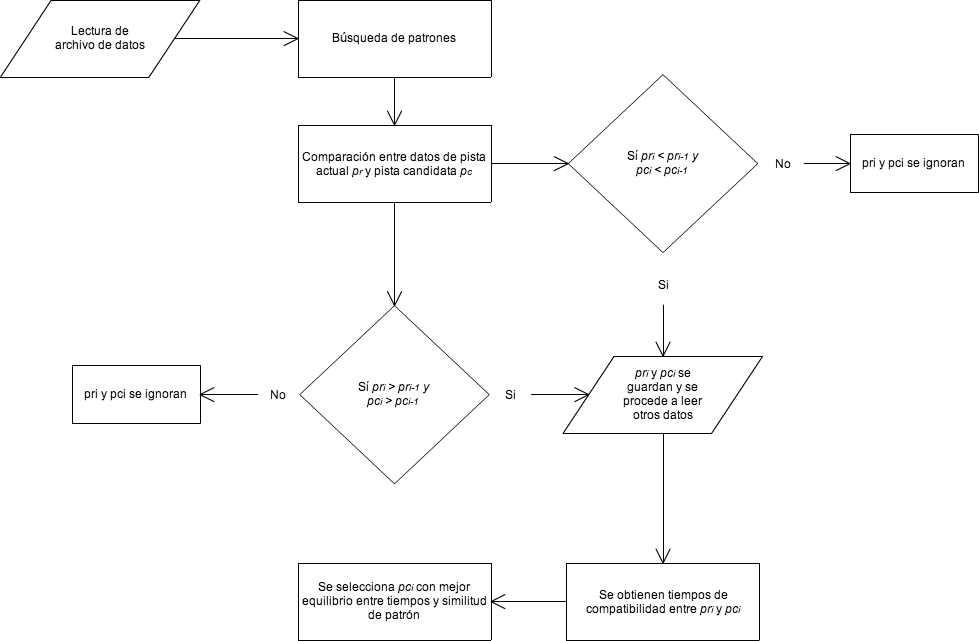
\includegraphics[width=22cm]{./Figuras/diagram3}
\caption[Generaci\'on de listas de reproducci\'on]{Diagrama que muestra la forma en que se generan las listas.}
\label{fig:diaglist}
\end{figure}
\end{landscape}
\section{Transici\'on inteligente entre pistas}

Una de los datos obtenidos del an\'alisis de la pista seleccionada es el tiempo en que ocurre el patr\'on encontrado, tanto en la pista actual como en la seleccionada, este dato describe el instante en la pista actual en que se puede iniciar una transici\'on de salida para la pista actual combinado con una de entrada para la nueva pista, de la cual tambi\'en se conoce el tiempo en que ocurrir\'ia la transici\'on.

\section{Dificultades}

Durante el desarrollo del proyecto presentaron varias dificultades; la b\'usqueda un m\'etodo eficiente para obtener datos de procesamiento, el intercambio de informaci\'on entre hilos sin afectar el flujo principal, efectuar transiciones sin perder informaci\'on de procesamiento entre pistas, entre otros problemas menores.

\noindent El principal problema fue el manejo de hilos en el programa; al realizar distintas actividades en el sistema operativo se generaban peque\~nas p\'erdidas de datos y pausas en la reproducci\'on que afectaban al an\'alisis. La soluci\'on fue utilizar subprocesos que corren de forma independiente del programa en segundo plano para evitar interferencias. Los subprocesos son programas independientes por lo tanto se pueden escribir en cualquier lenguaje distinto a la implementaci\'on principal, lo que aumenta la eficiencia en general.